\chapter{Introduction}
\label{chapter:introduction}

%\minitoc
\chapterwithfigures{\nameref*{chapter:introduction}}
%\chapterwithtables{\nameref*{chapter:introduction}}

\ifthenelse{\boolean{skipIntro}}{\endinput}{}

\section{Context}

\acf{AI} has been a subject of great interest for many decades, aiming at making machines reproduce more or less specific human behaviors, ranging from playing chess to producing medical diagnostics. Specifically, in the past decade, this domain has seen a rapid and almost exponential growth, being invested by numerous research labs and companies (like Google, Facebook, Microsoft, Amazon, etc.). Nowadays, applications of \ac{AI} are varied and show very impressive results. Those include information and image retrieval (web and image search engines), automatic translation, image recognition and classification (\eg Google Photos), face recognition, tracking of objects in videos, speech recognition, making autonomous vehicles drive, interpreting medical imagery, \etc.

One of the domains of \ac{AI} that shows the most impressive results is \acf{CV}, which focuses on automatic processing of images and videos. This domain is especially important considering the exponential growth of the volume of visual data being generated around the world, often uploaded and published on the Internet. For example, it is said that more than 500 hours of video are uploaded each minute on YouTube \citep{tubefilter} or 300 million new photos each day on Facebook \citep{zephoria}. Considering those figures, it is therefore clear that \ac{CV} is becoming more and more important to automatically process this large amount of data that would otherwise be impossible to handle by humans. In particular, \ac{CV} answers the necessity for those platforms to ensure a form of control on this content (\eg to prevent the upload of illegal material), but also the desire to propose new features and services related to this multimedia content (\eg captioning images for visually impaired people, or proposing semantic search in a photo library).

\begin{figure}[tb]
	\centering
	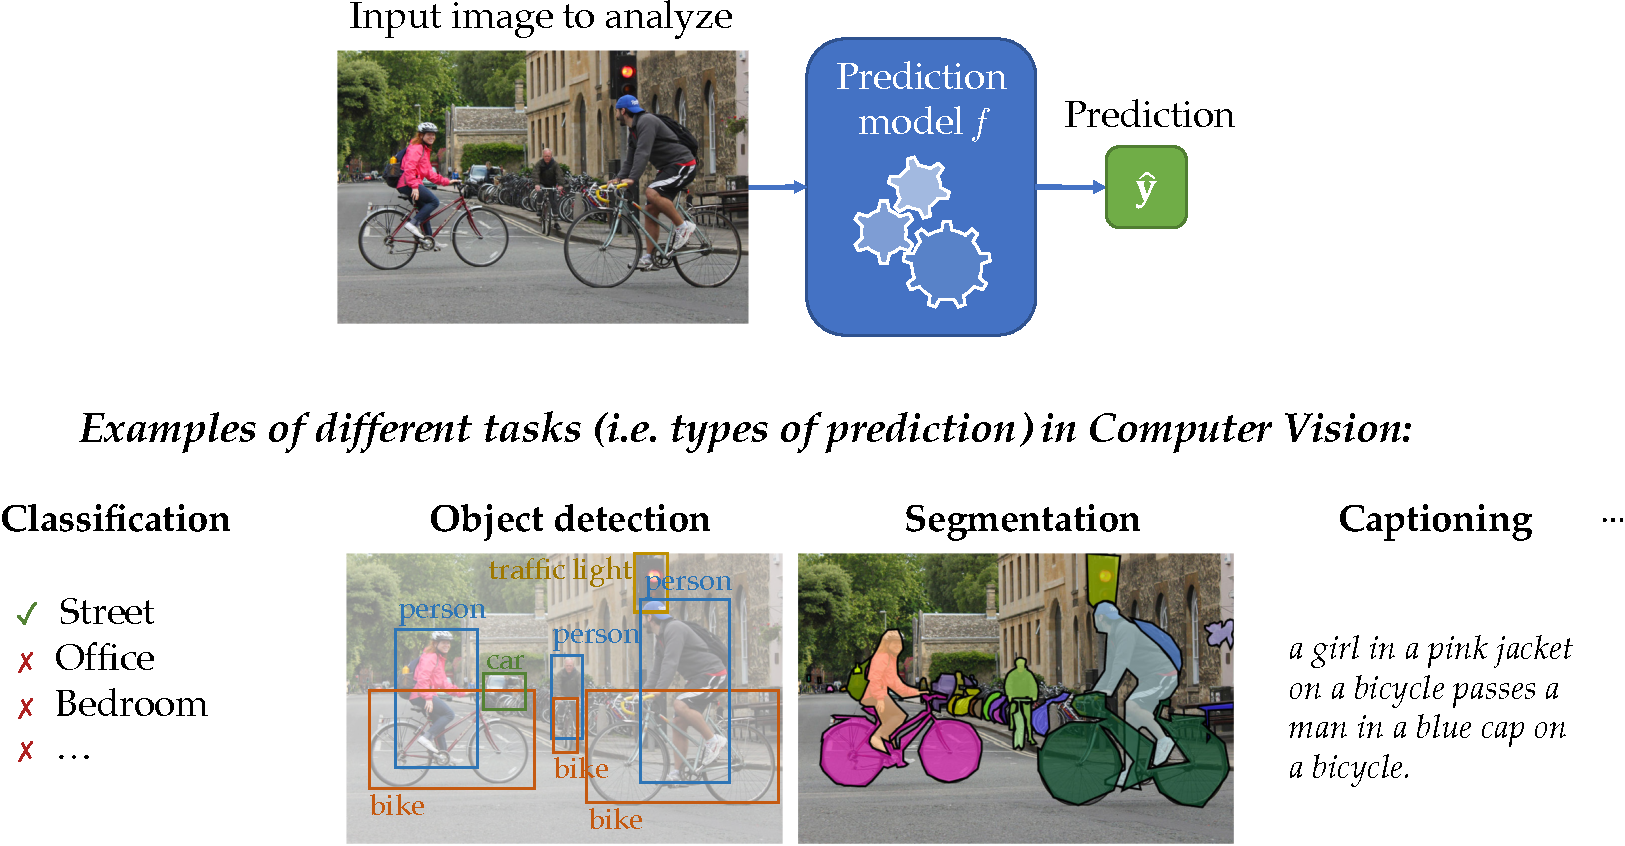
\includegraphics[width=\linewidth]{images/intro_CV}
	\titlecaption{General principle of \acf{CV}}{A discriminative model transforms an image into a prediction that depends on the task of interest. For example, classification, object detection (which usually implies localization of the object with a bounding box), image segmentation, image captioning, \etc}
	\label{intro:fig:CV}
\end{figure}

\acf{CV} aims at solving this issue and covers a lot of different tasks. We present the general principle and some of those tasks in \autoref{intro:fig:CV}: a predictive model $f$ transforms an input image into a prediction, that can be the class of the image, a list of objects and their localizations, a segmentation assigning a class to each pixel, a text caption, \etc. One particular problem with image data is what is called the ``semantic gap''. This describes the wide difference in meaning between what a human sees in a picture, \ie objects, concepts, a scene, \etc; and what a machine sees: pixel values, \ie numbers representing quantities of red, green and blue in quantized portions of space. For classification for example, a machine will need to \textit{bridge} this gap and find a mathematical mapping between pixel data and semantic categories.
%
To that end, \ac{CV} relies heavily on \acf{ML}, a broad domain that proposes to create models that learn to reproduce a task. To do so, these models use a dataset of examples to improve themselves until they produce satisfactory predictions. For example, given pictures of cats and dogs and knowing which one is on each picture, we can try to learn a model that distinguishes them.

To see how \ac{CV} evolved, we can take the example of the \acf{ILSVRC}, an image classification challenge created in 2010 based on a dataset of more than 1.2 million images (that later grew to 1.3 million) distributed among 1,000 classes used to train the \acf{CV} model. In the years 2010 and 2011, leading methods used a combination of handcrafted \ac{CV} preprocessing to find compact numerical representations of images, called features; and used \ac{ML} models to learn a mapping from those features to the possible classes of an image. This first step, called feature engineering, was long developed and refined and was a key component of the \ac{CV} field, allowing to partly bridge the semantic gap thanks to human knowledge in how pixels should be interpreted to form more meaningful representations, leaving the machine to learn a much simple task of mapping those meaningful representations to semantic classes. However, this step required specific handcrafting and expertise to find features that would best represent an image, requiring to be both robust and invariant to changes in the different images of a given class, while being different enough from one class to another to be able to correctly discriminate the classes.

In the year 2012, \acf{DL} models --\,a specific kind of \ac{ML} models\,-- started replacing this traditional approach and since that year, all winners of \ac{ILSVRC} are \ac{DL} models. \acf{DL} proposes to use a \acf{DNN} to transform the raw input data --\,pixels in the case of \ac{CV}\,-- into the desired semantic prediction, \eg the classes of \ac{ILSVRC}. This means that the traditional feature engineering step was replaced. With \ac{DL}, humans no longer design a smart way to transform the pixels, but rather design a framework of mathematical transformations and let the machine determine which features to extract from the raw data. Of course, because of this, \ac{DL} models need to be much more complex that the \ac{ML} models used before, with orders of magnitude more parameters that the machine needs to learn.

\begin{figure}[tb]
	\centering
	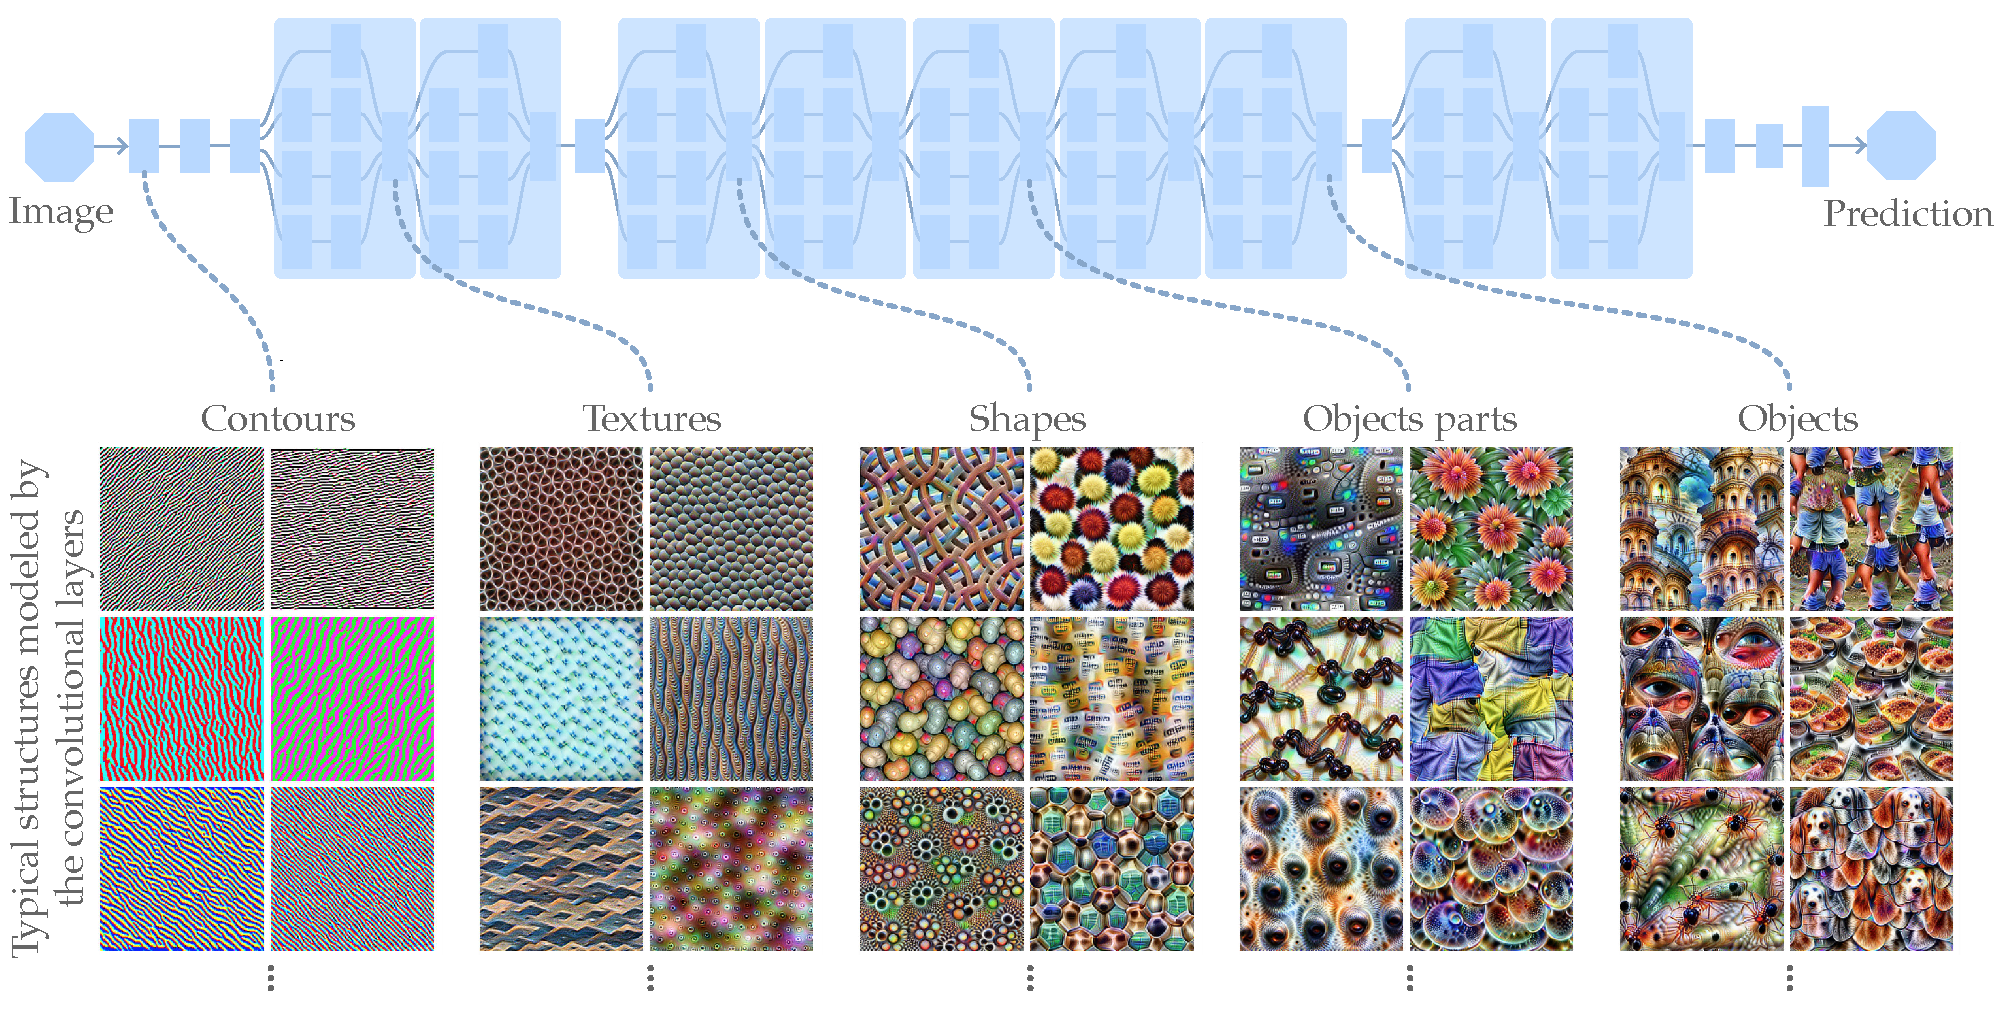
\includegraphics[width=\linewidth]{images/intro_CNN}
	\titlecaption{Illustration of the typical structures extracted by a \acs{ConvNet}}{The first layers detect simple contours, that are then assembled into textures, more complex shapes, parts of objects and finally complete objects. This property of representing more and more semantic information to finally produce a prediction arises thanks to the training of the \ac{ConvNet}. {\small Credits: Illustration based on \citet{olah2017feature}.}}
	\label{intro:fig:CNN}
\end{figure}

The type of \acf{DL} model that allowed \citet{alexnet} to win \ac{ILSVRC} in 2012 is a \acf{ConvNet}, a type of architecture especially well fitted for \ac{CV}. A \ac{ConvNet} produces a series of transformations of the input image into what is called \textit{latent} representations, until the final transformation produces the prediction. Interestingly, when investigating the information modeled by those representations \citep{olah2017feature} as illustrated in \autoref{intro:fig:CNN}, we can notice that a \ac{ConvNet} naturally learns to first detect contours, assembled in textures, shapes and object detections.

After 2012, \ac{DL} research has led to a succession of \ac{ConvNet} architectures each outperforming the previous one on \ac{ILSVRC}. It is also important to note that those deep \acp{ConvNet} designed for \ac{ILSVRC} have proven to be extremely versatile for \ac{CV} tasks, far beyond classification, and are now \textit{de facto} standards in the field. It is of course possible to use the same architecture to classify other datasets, and even take advantage of the features learned on ImageNet to obtain better results on much smaller datasets. But more interestingly, those architectures can be used as backbones for models used in many other \ac{CV} tasks such as object detection and localization \citep[\eg Faster R-CNN uses VGG-16, \textit{cf.}][]{ren2015faster}, segmentation \citep[DeepLab uses VGG-16 or ResNet-101, \textit{cf.}][]{chen2017deeplab}, \ac{VQA} \citep[MUTAN uses ResNet-152, \textit{cf.}][]{ben2017mutan}, \etc. This demonstrates the great strength and versatility of those models for \acf{CV}.

This \textit{revolution} of \acf{DL} was made possible by the combination of multiple factors. First of course, the progress in the architecture of the \acp{DNN} and in particular the development of \acfp{ConvNet}, started by \citet{nakamura} and refined over the years \citep{lecun1989backpropagation,alexnet,resnet}.
 Alongside the architecture, the training method of those models was also improved, with backpropagation methods first proposed by \citet{rumelhart1988learning,lecun} and refined as well to allow the training of those complex models \citep{dropout,batchnorm}. Finally, as we have seen, \ac{DL} models are much more complex than previous models. Their training was made possible thanks to large annotated datasets such as ImageNet \citep{imagenet}, the dataset of \ac{ILSVRC}; and the improvements of the computing hardware, especially the \acp{GPU}, strongly reducing the compute time required to train those models. Nowadays, pieces of hardware are even developed specifically for \ac{DL} training such as Google's \acp{TPU}.


\section{Motivations}

We now go over some interesting questions that remain open regarding the learning of \acp{ConvNet} for \acf{CV} and that we will tackle in the course of this thesis. Namely, regularizing \acp{DNN} is still an important problem, in particular because of their very large number of parameters. In this direction, using additional unlabeled data is an interesting solution addressed by \ac{SSL} for which further developments are interesting. Finally, producing more semantic and rich representations using disentangling is a new and interesting domain to address.

\paragraph{Regularization.} A key advantage of \acp{DNN} for \ac{CV} tasks is their large amounts of parameters that can model very complex transformations of the input image, which is necessary for complicated tasks. However, this is also an important problem since these models have orders of magnitude more parameters than there are images, even in large datasets like ImageNet and its 1.2M images. Because of this, deep \acp{ConvNet} easily suffer from over-fitting and require efficient regularization. In addition, the optimization problem of those \acp{DNN} is highly non-convex \citep{kawaguchi2016deep} which makes the training even more difficult. For these reasons, since the beginning of \ac{DL}, finding ways to make the training of those models possible has always been an important part of the research done by the community.

As such, numerous approaches have been developed over the years which became standard techniques. First, \acf{DA} \citep{dataaugmentation} tries to produce new images to artificially increase the size of the dataset; but is limited because it does not really produce new information. Numerous techniques are also based on adding noise at different stages of the training process \citep[\textit{cf.}][]{kukavcka2017regularization}, which have shown to help generalization but have a behavior that is not really interpretable and thus provide no control over it. A popular type of noise injection is dropout \citep{dropout} and its variants, which disconnects parts of the model randomly. While some interpretations exist, the exact advantage obtained by disabling parts of the model is not obvious, seems unnatural, and fails on some architectures. Weight decay \citep{weightdecay} is also a popular regularization technique that is equivalent to L2 regularization of non-\ac{DL} models. While for linear models it encourages smoother decision function, its effect with deep networks is less clear \citep{rethinking}. Finally, the very popular \acf{BN} \citep{batchnorm} has recently been key to train very deep \acp{ConvNet} like ResNet, but the interpretation of its behavior is currently debated in the community \citep[\textit{cf.}][]{santurkar2018does}. \citet{zhang2019fixup} even recently proposed to simply replace it with a simple specific weight initialization that provides equivalent results. Those numerous limitations in our understanding of how those existing techniques affect the generalization performance of \acfp{DNN} are studies by \citet{rethinking}. They conclude, ``explicit regularization may improve generalization performance, but is neither necessary nor by itself sufficient for controlling generalization error''.

\paragraph{\acl{SSL}.} Another interesting aspect of the \ac{DL} literature is \acf{SSL} which proposes to use partially labeled datasets. As we have seen, \ac{DL} usually relies on large labeled datasets which are costly to obtain; something that \ac{SSL} tries to limit by using a mostly unlabeled dataset, only using a small number of labeled images for each class. To that end, two main categories of techniques exist: invariance-based methods and reconstruction-based methods.

Invariance-based methods rely on producing latent representations that are well fitted for classification. In particular, \citet{Sajjadi2016,Laine2016,Tarvainen2017} propose to enforce the stability of the class prediction for different versions of the same image. Reconstruction-based methods use an unsupervised reconstruction loss to extract additional information from unlabeled images, producing features that are more robust, more general and representative of the full diversity of the data \citep{Ranzato2008}. We can see that the first technique aims at improving the invariance of the features while the second aims at improving their representativity.

While both are interesting and could seem complementary, they pose the problem of having conflicting roles. The first idea aims at improving classification directly by increasing the invariance and discriminative nature of the representations. On the other hand, reconstruction proposes to extract features regardless of their ability to discriminate the supervised task that we eventually want to solve. This means that even if reconstruction would improve the quality of the discriminate features, it would also extract numerous features that are not well fitted for classification.


\paragraph{Disentangling.} Finally, an interesting domain of research called \textit{disentangling} proposes to look for ways to improve the semantic quality of the latent representations of \acp{DNN}. The definition of disentangling varies \citep{higgins2018towards} but it mostly aims at producing representations that model independent factors of variation of the data. For example, considering a dataset of faces, we would like to have independent representations of the hairstyle, the makeup, the smile, the eye colors, the presence of glasses, \etc. This kind of models try to improve the quality of the features that can then be used for various semantic tasks (classification, retrieval, \etc) or to interpret and manipulate the representation of an input.

A first solution is to address disentangling in an unsupervised manner, meaning that no label regarding the factors of variation of the dataset are provided. Those models, in particular $\beta$-\acs{VAE} \citep{higgins2017beta} and its variations \citep{chen2018isolating,Klys2018}, are effective at providing features that are independent of each other. However, because no label is used, they are not able to provide semantic information about the factors they extracted. In addition, the absence of labels does not encourage the representation of complex semantic factors and is more likely to produce simpler low-level variations that possess limited semantic information.

The second solution is to rely on labels of factors of variation. This can be done using conditional generative models \citep{perarnau2016invertible,Lample2017} but this has the drawback of representing the labeled factors in a binary state, which is usually not sufficient since it is impossible to encode the complex diversity of those factors with only one boolean. Other approaches propose to use latent subspaces to represent and disentangle different kinds of semantic information. \citet{Mathieu2016,Hadad2018,Liu2018a} for example all propose to use a latent space split in two parts, each dedicated to an information domain, \eg the identity of a person on one side and its visual attributes (hairstyle, makeup, \etc) on the other. Using labels, they can provide semantic information but usually rely on labels for one of the two types of information which is the cause of most of their limitations as we will see.


\section{Contributions and outline}

Because \ac{DL} now produces classification scores comparable to human performance using very large models on ImageNet, in this thesis, we propose to study \acp{ConvNet} ``beyond ImageNet'', investigating and improving the capabilities of those models beyond proposing bigger and deeper architectures on extremely large datasets. In particular, we know that \acp{ConvNet} produce a succession of representations encoding pieces of information extracted from the input. We propose to investigate in depth different ways to improve the quality of those representations. First, by improving their discriminative quality using invariance-based regularization. Then, dealing with fewer labels and additional unlabeled data, we propose new architectures to structure the latent space for \acf{SSL}. This structuring of the information is then pursued and reinforced to address the disentangling of complementary information.

\acused{SHADE}
\begin{itemize}
	\item \autoref{chapter:shade}: \nameref{chapter:shade}\\
	We first propose an overview of the recent evolution of \ac{DL} and deep \acp{ConvNet} and position the work of this thesis regarding regularization, \ac{SSL} and disentangling of \acp{DNN}.

	We then propose our contribution, a new regularization method called \textbf{\acs{SHADE}}. This method is inspired by recent work applying the \ac{IB} principle to \acp{DNN}. With \acs{SHADE}, we explicitly work on influencing the information represented  by a \ac{DNN}. Because an input image contains a very large amount of information, from which only a small portion is relevant for classification, we propose to encourage the filtering of such information.
	Representations should indeed be intra-class invariant, filtering out all the inherent variability of each category to focus on discriminate information only. 
	To explicitly encourage this intra-class invariance, \acs{SHADE} minimizes the entropy of the representations conditionally to the classes. This optimization goal is both interpretable and perfectly aligned with the goal of classification. We demonstrate its effectiveness at producing more robust and invariant features using different standard architectures on CIFAR-10.


	\item \autoref{chapter:hybridnet}: \nameref{chapter:hybridnet}\\
	In this chapter, we focus on improving standard deep \acp{ConvNet} using \acf{SSL} by working on the way latent information is structured in this context.
	%
	Current \ac{SSL} methods seem to have conflicting objectives and cannot work in synergy, with classification and stability methods increasing the invariance of the representations, filtering only the discriminative information; while reconstruction requires to conserve all the information to reach its goal. Thus, when mixing classification with reconstruction arises a dilemma.
	
	To overcome this conflict and overcome this ``incompatibility'', we introduce a novel idea to structure the information in two separate and complementary latent spaces. This takes the form of a novel architecture and a dedicated training method called \textbf{HybridNet}. This architecture uses an encoder with two branches so that the first branch can encode only the discriminative information and is allowed to remove the rest of the information, which is captured by the second branch and therefore allows correct reconstruction of the image. Thanks to this, we make reconstruction, classification and invariance regularization work in cooperation instead of in opposition. We validate the effectiveness of our method compared to the state of the art on CIFAR-10, SVHN and STL-10. We also propose in-depth analysis of the different terms of the loss as well as visualizations to gain insight regarding the behavior of the model.


	\item \autoref{chapter:dualdis}: \nameref{chapter:dualdis}\\
	Finally, in an attempt to pursue our work on organizing and separating information in complementary latent spaces, we address the problem of disentangling factors of variation.
	We propose to design a model that separates two complementary types of information that we call \textit{information domains}; for example, with a dataset of faces, the first domain is the identity (\ie the \textit{class}) of the person and the second is the visual \textit{attributes} (hairstyle, makeup, \etc).

	For this, we develop a framework called \textbf{DualDis}, which relies on a two-branch architecture, each domain being assigned to one branch. Using adversarial training \citep{Goodfellow2014}, we explicitly train the model to disentangle the two domains so that their information is contained in one branch only. Using classifiers, we structure the representation space in order to be able to efficiently manipulate it, enabling simple semantic image editing and generation of new images. We validate this model on CelebA, Yale-B and NORB with a comparison to the state of the art and examples of possible applications of such an architecture, namely image editing and generation of images for data augmentation.
\end{itemize}

We conclude this thesis in \autoref{chapter:conclusion} and discuss several interesting directions for future work.

\section{Related publications}

This thesis is based on the material published in the following papers:
\begin{itemize}
	\item \fullcite{Blot2018}, best paper award;
	\item \fullcite{Robert2018};
	\item \fullcite{Robert2019}.
\end{itemize}
